\chapter{\IfLanguageName{dutch}{Stand van zaken}{State of the art}}
\label{ch:stand-van-zaken}
\graphicspath{{../../Images/}} 
% Tip: Begin elk hoofdstuk met een paragraaf inleiding die beschrijft hoe
% dit hoofdstuk past binnen het geheel van de bachelorproef. Geef in het
% bijzonder aan wat de link is met het vorige en volgende hoofdstuk.

% Pas na deze inleidende paragraaf komt de eerste sectiehoofding.

%%Dit hoofdstuk bevat je literatuurstudie. De inhoud gaat verder op de inleiding, maar zal het onderwerp van de bachelorproef *diepgaand* uitspitten. De bedoeling is dat de lezer na lezing van dit hoofdstuk helemaal op de hoogte is van de huidige stand van zaken (state-of-the-art) in het onderzoeksdomein. Iemand die niet vertrouwd is met het onderwerp, weet nu voldoende om de rest van het verhaal te kunnen volgen, zonder dat die er nog andere informatie moet over opzoeken \autocite{Pollefliet2011}.

%%Je verwijst bij elke bewering die je doet, vakterm die je introduceert, enz. naar je bronnen. In \LaTeX{} kan dat met het commando \texttt{$\backslash${textcite\{\}}} of \texttt{$\backslash${autocite\{\}}}. Als argument van het commando geef je de ``sleutel'' van een ``record'' in een bibliografische databank in het Bib\LaTeX{}-formaat (een tekstbestand). Als je expliciet naar de auteur verwijst in de zin, gebruik je \texttt{$\backslash${}textcite\{\}}.
%%Soms wil je de auteur niet expliciet vernoemen, dan gebruik je \texttt{$\backslash${}autocite\{\}}. In de volgende paragraaf een voorbeeld van elk.

%%\textcite{Knuth1998} schreef een van de standaardwerken over sorteer- en zoekalgoritmen. Experten zijn het erover eens dat cloud computing een interessante opportuniteit vormen, zowel voor gebruikers als voor dienstverleners op vlak van informatietechnologie~\autocite{Creeger2009}.
%\newpage
\section{Versiebeheer}
\subsection{Inleiding}
\label{sec:vb_inleiding}
Versiebeheer is een belangrijk concept binnen softwareontwikkeling. Zo waren er in 2018 in het  totaal 100 miljoen projecten op het populaire versiebeheer platform GitHub \autocite{Git2018}. GitHub (sinds 2018 overgenomen door Microsoft) is niet de enige speler op de markt. Er zijn ook nog Code Commit van Amazon en GitLab. Veel bedrijven spelen dus in op de behoefte aan een duidelijk en efficiënt versiebeheersysteem. De vraag stelt zich dan ook: welke behoefte lossen deze systemen op?

Stel volgende scenario voor: Alice en Bob zijn aangenomen om te werken voor bedrijf X. Hun eerste taak is een website ontwikkelen. Ze leggen samen alle vereisten vast, bespreken de verschillende technologieën en gaan aan de slag. Op het einde van de eerste dag hebben ze elk een verschillende pagina gemaakt die ze graag met elkaar delen willen delen. Dit kan door bijvoorbeeld via mail de bestanden door te sturen. Een andere mogelijkheid is de bestanden via fysieke hardware zoals een USB-Stick aan elkaar te geven. Het nadeel is dat de code op twee verschillende plaatsen verspreid zit. Als Bob de code kwijt raakt dan zal deze opnieuw moet worden geschreven. Om dit probleem te voorkomen kan men het project op een centrale server opslaan. Bob en Alice zullen hun veranderingen opslaan op deze centrale server. Zo hebben ze altijd toegang tot elkaars werk. 

Deze manier van werken heeft nadelen. Alice kan per ongeluk een bestand overschrijven of een stuk code verwijderen. Tenzij er back-ups zijn is het originele bestand verloren. Om dit probleem te omzeilen wordt er gebruik gemaakt van het concept van \textbf{versies}. Elke aanpassing die er gemaakt wordt resulteert in een nieuwe versie van het project. Men kan altijd terugkeren naar een eerdere versie. Als Alice dus het stukje code verwijdert in versie 15 kan men terug naar versie 14.

\textcite{Loeliger2009} stelt dat een versiebeheersysteem een middel is om verschillende versies van code te beheren en bij te houden. De auteur onderscheidt volgende drie eigenschappen waaraan dergelijke systemen voldoen:

\begin{itemize}
	\item er wordt gebruik gemaakt van een centraal archief. Binnen dit archief worden alle versies van het project bewaard en bijgewerkt.
	\item het centraal archief geeft toegang tot eerdere versies van het project.
	\item alle veranderingen die worden aangebracht aan het archief worden genoteerd in een centraal logboek.
\end{itemize}

Versiebeheer is geen nieuw concept. Er zijn zoals eerder aangehaald verschillende software oplossingen beschikbaar. Volgens \textcite{Chacon2014} zijn er drie grote categorieën (zie \ref{fig_types_cvs} voor een grafische weergave):

\begin{itemize}
	\item lokale versiebeheersystemen: het centraal archief waar de veranderingen in worden bewaard, staat op een lokale computer. Het grootste voordeel is dat een lokaal systeem zeer makkelijk te onderhouden is en eenvoudig op te stellen. Toch is het niet geschikt om bestanden met elkaar te  delen of samen aan bestanden te werken. Een gekend voorbeeld is RCS (Revision Control System) - zie \ref{sec:RCS} -. \\
	
	\item CVCS: om samen te kunnen werken aan dezelfde bestanden kan een CVCS (Centralised Version Control System) worden gebruikt. In plaats van het archief lokaal bij te houden wordt er gebruik gemaakt van een centrale server. Bestanden worden vervolgens lokaal gekopieerd. Als er veranderingen worden aangebracht zullen deze worden doorgestuurd naar de server.Doordat men verplicht is om de bestanden op een centrale plaats af te halen, kan men deze afschermen. Zo kan men de toegang beperken tot enkel de nodige bestanden per gebruiker. \\
	
Een neveneffect van alles centraal te beheren is het zogenaamde \textit{single point of failure (SPOF)} probleem. Een SPOF is een onderdeel van een systeem dat mocht het uitvallen heel het systeem tot een halt roept. Met andere woorden valt het centraal archief weg heeft niemand nog toegang tot het project. Een mogelijke oplossing voor dit probleem is redundantie. Dit betekent het aanbieden van kopieën. \autocite{Sun2007}\\

	\item DVCS: om het SPOF probleem te voorkomen kan men kopieën maken van het centraal archief. Deze kopieën kunnen vervolgens worden verspreid over verschillende computers. Dit is het uitgangspunt van DVCS (Distributed version control System). Elke gebruiker heeft een lokale kopie van de centrale server. De veranderingen aan de bestanden worden eerst aangebracht in het lokaal archief en vervolgens gesynchroniseerd met de centrale variant.\\

Mocht het centraal aanspreekpunt niet beschikbaar zijn is dit geen probleem. Elke gebruiker heeft immers een volledige back-up van het volledige project. In theorie kan de gebruiker zelfs optreden als nieuwe centrale server.
\end{itemize}


\begin{figure}[h!]
	\centering
	\begin{subfigure}[b]{.5\textwidth}
	\centering
		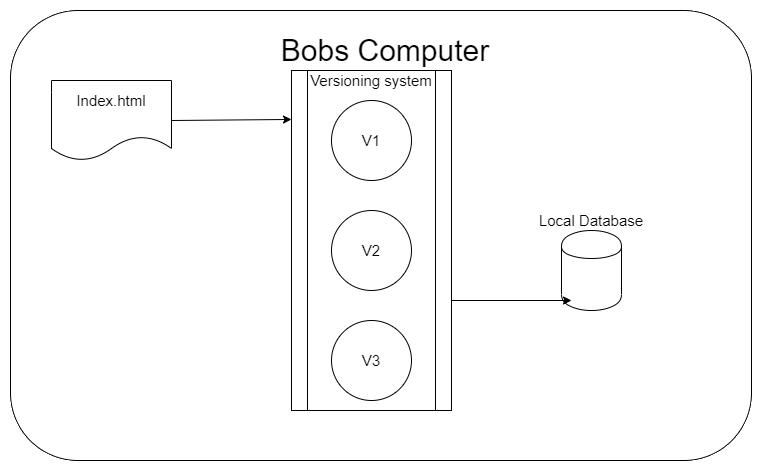
\includegraphics[scale=.3]{LVCS.png}
		\caption[Overzicht structuur Lokale VCS]{Overzicht van de structuur van een Lokale VCS.}
	\end{subfigure}%
	\begin{subfigure}[b]{.5\textwidth}
	\centering
		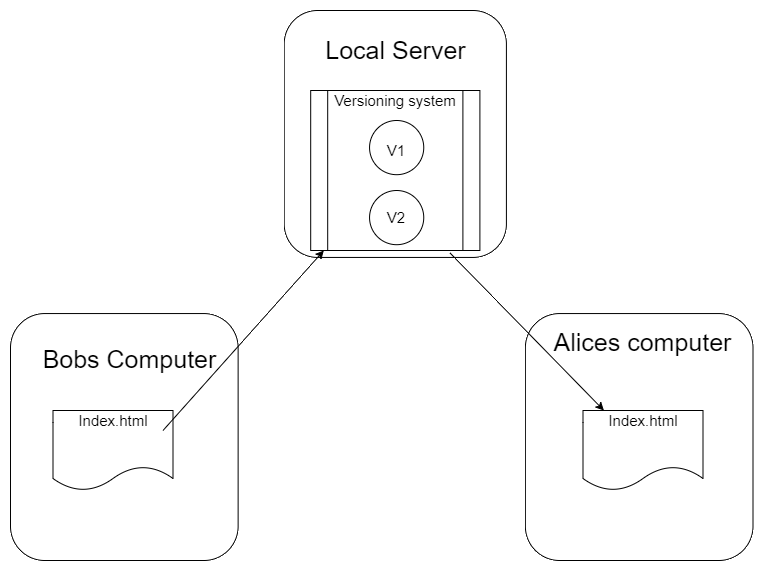
\includegraphics[scale=.3]{CVCS.png}
			\caption[Overzicht structuur CVCS]{Overzicht van de structuur van een CVCS.}
	\end{subfigure}%
	\hfill
	\begin{subfigure}{.5\textwidth}
		\centering
		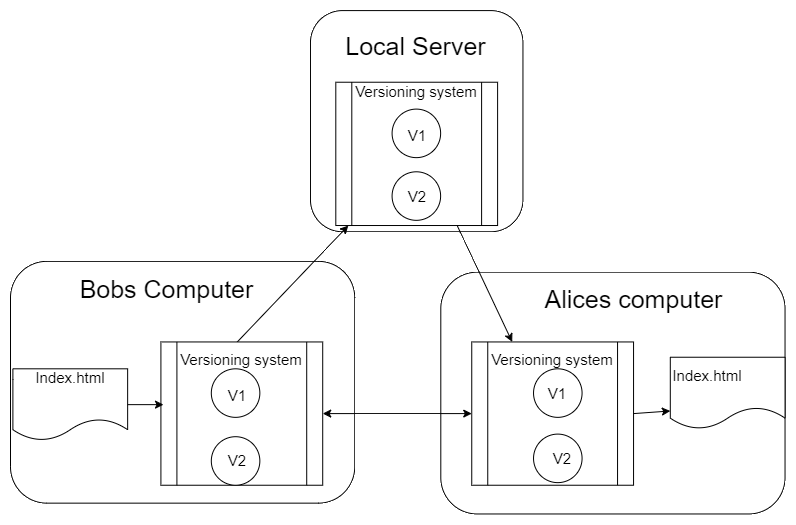
\includegraphics[scale=0.3]{DVCS.png}
	\caption[Overzicht structuur DVCS]{Overzicht van de structuur van een DVCS.}
	\end{subfigure}
	
	\caption[Overzicht types VCS]{Overzicht van de drie types van VCS zoals aangegeven door \textcite{Chacon2014}.}\label{fig_types_cvs}
\end{figure}

	
\subsection{RCS}
\label{sec:RCS}


RCS \textit{(Revision Control System)} is een lokaal versiebeheer systeem. Het wordt voor het eerst beschreven in een artikel geschreven door \textcite{Tichy85rcs}. Het werd verder ontwikkeld binnen het GNU project -Een open source besturingssysteem \footnote{GNU is veel meer dan enkel open source. Het GNU project is sterk verbonden met de ideologie en organisatie van de free software foundation (FSF). Meer informatie omtrent deze organisatie en beweging is te vinden op: \url{https://www.fsf.org/}}- waar het als vervanging voor het CSSC Systeem \autocite{GNUCSSC} werd gebruikt. CSSC is een systeem gebaseerd op SCCS (Source code control system) dat ontworpen is voor UNIX systemen. SCCS is in opdracht van Bell Labs ontwikkeld door \textcite{Rochkind1975}.\\

Voordat RCS op de markt kwam is er nog tal van andere software ontwikkeld. Zo was er CA-Panvalet een gepatenteerde oplossing voor Mainframe computers.\\

Waarom is het interessanter om RCS in detail te bekijken? Veel van de concepten waar het gebruik van maakt zijn aanwezig in moderne systemen (zoals GIT). Het is open source en wordt nog steeds op vrijwillige basis onderhouden, wat aansluit bij de visie van deze bachelorproef.\\

De manier waarop versies worden bijgehouden in RCS -zoals door \textcite{Tichy85rcs} beschreven- is gebaseerd op een boomstructuur -denk aan een stamboom-. Volgens \textcite{Lievens2019}, is een boom een collectie van \textbf{toppen} \textit{(in het Engels ook wel Nodes genoemd)}. Deze toppen hebben een hiërarchische verband.Zo bestaat er bijvoorbeeld een kind-ouder verband. Er zijn twee bijzondere toppen in een boom:

\begin{itemize}
	\item de wortel(\textit{root}): Deze top ligt helemaal aan het begin van de boom. Alle andere toppen zijn afstammelingen van deze top. Het heeft aldus geen ouders.
	\item een blad(\textit{leaf}): Deze top heeft geen kinderen. In tegenstelling tot een wortel kunnen er meerdere bladeren aanwezig zijn.
\end{itemize}

Alle andere toppen worden intermediair genoemd. Elke top heeft mogelijk een aantal kinderen. De diepte van de wortel is nul ($d$=1) en elk kind heeft als diepte: Elk van deze kinderen is op zijn beurt de wortel voor een nieuwe deelboom. Het concept van \textbf{diepte} is belangrijk. 

\begin{equation}
	d_{kind} = d_{ouder} + 1
\end{equation}

%vervang met referentie
Al deze concepten worden ook nog eens grafisch verduidelijkt in de figuur \ref{fig_tree}.

\begin{figure}[h!]
\centering
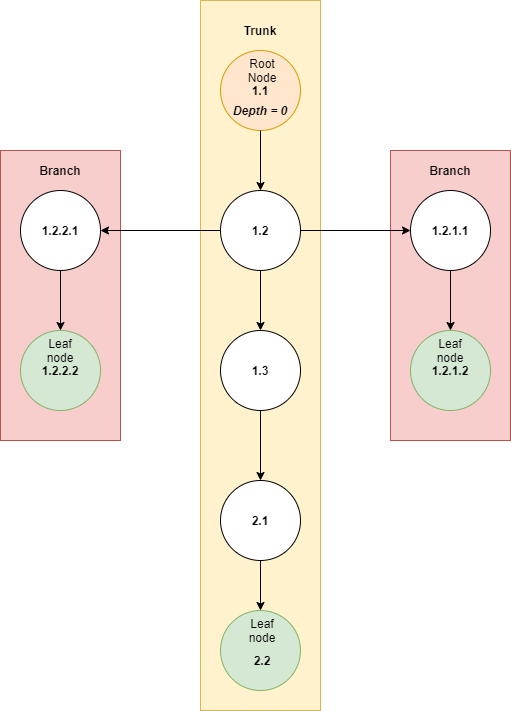
\includegraphics[scale=0.5]{tree1.png}
\caption[Overzicht concepten boomstructuur]{Een overzicht van alle concepten binnen een boomstructuur waar RCS van gebruik maakt.}\label{fig_tree}
\end{figure}

Er kan gebruik gemaakt worden van een boomstructuur om de onderlinge relaties tussen de versies weer te geven. Stel: Bob en Alice zijn bezig aan de hoofdpagina. Bob maakt een initiële versie van de pagina. Vervolgens wilt hij die graag delen met Alice. Hiervoor gebruikt hij het commando om een nieuwe versie aan te maken\footnote{\Verb+ci homepage.html+}. Dit commando wordt \textbf{inchecken} genoemd. Binnen GIT is dit vergelijkbaar met het commando \textit{git push}. Aangezien dit de eerste versie is kan men dit vergelijken met het aanmaken van een wortel. Volgende versies worden kinderen van de vorige versie. Zo wordt versie 1.4 kind van versie 1.3. Inchecken gaat niet alleen onze boomstructuur aanmaken maar ook de extensie \textit{.v} toevoegen (\verb+homepage.html.v+). Het originele bestand wordt ook verwijderd\\

Het bestand krijgt ook een \textbf{versienummer}. Dit versienummer heeft de vorm: $x_1.x_2$.\ $x_1$ (ook wel \textit{release} genoemd) staat voor een grote verandering. Bijvoorbeeld het in productie nemen van een nieuwe versie.$x_2$ (\textit{level}) staat voor een kleinere verandering. Een andere manier om $x_2$ te bekijken is de diepte met als wortel de laatste release ($x_1$). 1.1 is het versienummer van de wortel die Bob heeft aangemaakt. 1.4 is het derde kind van de wortel.Elke check-in zal het level ($x_2$) met één verhogen. Het release nummer ($x_1$) wordt manueel verhoogd door middel van de \textit{-r} optie bij check-in \footnote{\Verb+ci -r2 homepage.html+}. Bij branches is er ook nog spraken van $x_3$ en $x_4$ zie \ref{par:branches}.\\

Deze manier van versies te bestempelen wordt nog steeds gebruikt. Het is echter niet de enige manier. \textit{Semantic versioning} is een gekend alternatief. Het concept van versienummers bestaat in Git onder de vorm van \textit{tags} (\ref{sec:GIT}).\\

Er is nu een bestand onder de vorm \verb+homepage.html.v+. Hoe kan Alice nu dit bestand aanpassen en een nieuwe versie publiceren? Alice zal het bestand moeten \textbf{uitchecken}.Dit kan ze doen door middel van het commando \verb+co+ en de naam van het bestand \footnote{(\Verb+co homepage.html+)} . Het uitchecken is aldus het verkrijgen van een specifieke versie uit het archief. Als er geen specifieke versie wordt meegegeven wordt de laatste versie opgehaald. Om een specifieke versie op te halen kan er gebruik gemaakt worden van de optie -r  \footnote{(\Verb+co -r1.1 homepage.html+)} . Alice heeft nu een kopie van het originele bestand gekregen. Merk op dat in tegenstelling tot inchecken ons archief niet wordt verwijderd. Vervolgens kan ze in deze lokale kopie wijzigingen aanbrengen. Tot slot wordt het bestand weer aan het lokaal archief toegevoegd door middel van inchecken. Het equivalent van \verb+co+ binnen git is \verb+git pull+.\\

\begin{wrapfigure}{r}{0.5\textwidth}
\begin{center}
  	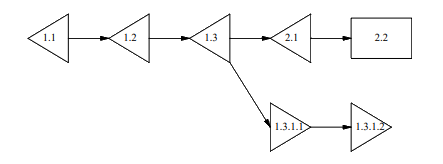
\includegraphics[scale=0.6]{deltas.png}
\end{center}
\caption[Voorbeeld van deltas.]{Een voorbeeld van deltas.De Trunk bevat een series van achterwaardse deltas terwijl alle branches enkel voorwaardse deltas bevatten. Grafiek afkomstig uit \textcite{Tichy85rcs}}\label{fig_deltas}
\end{wrapfigure}

Hoe worden de verschillen tussen de versies bijgehouden in ons lokaal archief? Een mogelijke oplossing zou zijn om alle versies van het bestand afzonderlijk bij te houden. Dit vraagt veel opslagruimte. RCS gebruikt voor dit probleem het concept van \textbf{deltas}. Een delta houdt bij welke regels veranderd zijn ten opzichte van de vorige versie. Doordat de delta enkel de relevante lijnen bijhoudt wordt de opslag beperkt \footnote{De delta wordt opgebouwd aan de hand van het GNU commando diff \url{https://www.gnu.org/software/diffutils/}}. Er zijn twee types van deltas: \textbf{voorwaardse deltas} en \textbf{achterwaardse deltas}. Bij het inchecken van een nieuwe versie zal de vorige versie worden vervangen door een achterwaardse delta. Zit men momenteel op versie 1.3 en  vraagt men versie 1.2 dan zal de achterwaardse delta van versie 1.2 worden toegepast op versie 1.3. (Voorwaardse deltas komen aan bod in het gedeelte over branching (\ref{par:branches}). Het concept van deltas wordt nog eens verduidelijkt door een voorbeeld in de appendix -zie \ref{ch:voorbeeld-rcs}-.)\\

Inchecken en uitchecken ligt aan de basis van het archiefsysteem. Toch is er nog een probleem aanwezig met deze manier van werken. Stel dat Alice en Bob gelijktijdig wijzigingen aanbrengen aan een bestand. Ze willen dit bestand elk afzonderlijk publiceren.  Hierdoor ontstaan er twee versies die afstammen van één gezamenlijke versie. De boomstructuur wordt in twee gesplitst. Dit is niet mogelijk aangezien een versie altijd uniek moet zijn. Hoe kan men verzekeren dat elke versie slechts één kind heeft (op dezelfde branch)? Dit probleem wordt opgelost door \textbf{sloten}(engels=lock).Dit concept geeft gebruikers de mogelijkheid om een versie te  versleutelen. Terwijl een versie versleuteld is kan niemand anders wijzigingen aanbrengen. Andere gebruikers kunnen deze nog bekijken. Op het moment dat Bob zijn versie gaat uitchecken kan hij deze versleutelen (door middel van de \textit{-l} optie bij het co commando). Hierdoor kan Alice geen nieuwe versie meer aanmaken tot Bob zijn wijzigingen heeft doorgevoerd. Met andere woorden zolang Bob het slot niet vrijgeeft kunnen er geen nieuwe versies worden aangemaakt\footnote{In sommige gevallen kan het slot ook worden 'geforceerd' mocht Bob bijvoorbeeld ziek vallen}. Deze manier van werken heeft een zichtbaar nadeel. Alice is verplicht om te wachten op Bobs nieuwe versie alvorens ze veranderingen kan aanbrengen. Git gebruikt het concept van sloten niet. Daar maakt men gebruik van \textbf{merges} om dit zelfde probleem aan te pakken %\ref{sec:GIT}%.

\subsubsection{Opmerkingen}
In het originele artikel wordt de klemtoon gelegd op het onderling delen van de verschillende versies. Hierdoor kan men de indruk krijgen dat er een centrale server betrokken is. Dit is niet het geval. De software is ontworpen om op één besturingssysteem uitgevoerd te worden. Volgens \textcite{Debian2020} is GNU aangezien het gebaseerd is op UNIX een \textit{multi-user os}. Dat wil zeggen dat meerdere gebruikers het systeem tezelfdertijd kunnen gebruiken door middel van een terminal connectie. Hierdoor kan men onderling de bestanden delen ondanks dat men niet gaat werken in een CVCS.

\subsection{branches}
\label{par:branches}
\subsubsection{Duiding}
Door het principe van sloten en inchecken lijkt het alsof elke versie exact één opvolger heeft. Zo zal versie 1.3 de opvolger zijn van 1.2. Toch kunnen er zich zoals in een stamboom  vertakkingen voordoen. De vertakkingen worden \textbf{Branches} genoemd. De hoofdboom (niet vertakte toppen die afstammen van de wortel) wordt de \textbf{trunk} genoemd. Dit principe kan men het best demonstreren aan de hand van een figuur. Zo kan men zien in figuur \ref{fig_tree} dat er twee vertakkingen zijn op versie 1.2. Het principe van vertakkingen lijkt op het eerste zicht complex en onoverzichtelijk. \textcite{Tichy85rcs} geeft enkele redenen om dit toch toe te passen.

\begin{enumerate}
\item Doorvoeren van veranderingen in oude versies: Stel dat een bedrijf een oude versie van een software product gebruikt. Dit product is ontwikkeld met behulp van RCS. Er wordt een fout in deze oude versie gevonden die om een oplossing vraagt. Aangezien er in de tussentijd nieuwere versies zijn is dit niet evident. Het bedrijf zou volledig moeten overstappen op de nieuwste versie alvorens een aanpassing kan gebeuren. Om deze situatie te vermijden kan men gebruik maken van vertakkingen. Zo kan men een vertakking maken op de gewenste versie en kleine aanpassingen doorvoeren.\\
\item Andere implementaties: stel dat een ontwikkelaar een nieuw stuk code wilt uittesten. Deze heeft niet het gewenste resultaat. Mocht dit stuk code bewaard worden op de hoofdboom (\textit{trunk}) dan is er een onstabiele versie gepubliceerd. Een gebruiker die op dat moment de recentste versie opvraagt, krijgt dus een niet werkend product.\\
Door branches te gebruiken kan men ervoor zorgen dat er enkel werkende versie op de hoofdboom terecht komen. Nieuwe stukken code worden eerst geïsoleerd en getest alvorens opgenomen te worden. Op die manier blijft het archief in een overzichtelijke en stabiele vorm.
\end{enumerate}

\begin{wrapfigure}{L}{0.5\textwidth}
\begin{center}
  	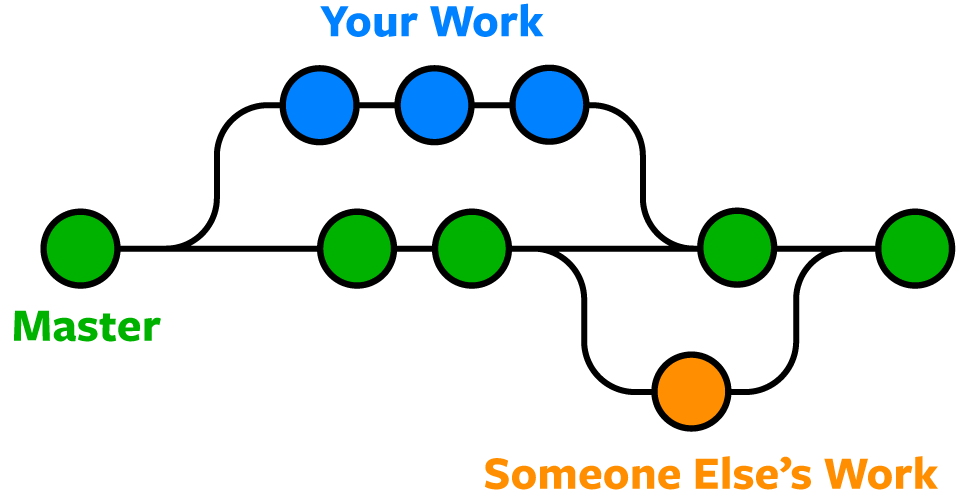
\includegraphics[scale=0.2]{git-branches-merge.png}
\end{center}
\caption[Voorbeeld merge proces.]{Een voorbeeld van een merge proces. Eerst wordt er een branch aangemaakt die na drie versies terug in de master wordt gemerged. Grafiek gepubliceerd door \textcite{NobleDesktop2018}}\label{fig_merge}
\end{wrapfigure}

Door middel van vertakkingen kan code worden geschreven en de hoofdboom stabiel gehouden. Zelfs met veel ontwikkelaars en grote projecten kan men door deze manier van werken code conflicten vermijden. Eenmaal de code klaar is voor productie kan men deze gaan publiceren op de hoofdboom. Dit concept wordt ook wel \textbf{mergen} genoemd. Dit principe wordt geïllustreerd door de figuur \ref{fig_merge}.

%todo uitleg van RCS branching en forward deltas

\subsubsection{Flows}
Er is echter nog een grote vraag die niet beantwoord is: wanneer moet men gaan vertakken?

De eerste reden aangehaald door \textcite{Tichy85rcs} -het doorvoeren van veranderingen- is minder relevant binnen de context van DVCS. Er wordt namelijk niet meer op een gezamenlijk archief gewerkt maar op een lokale kopie. Het bedrijf kan dus op zijn eigen kopie lokaal veranderingen aanbrengen .De tweede reden is echter wel belangrijk. Stel dat een project honderden bestanden en ontwikkelaars heeft. In zo een omgeving kunnen veranderingen soms onvoorspelbare gevolgen hebben. Ontwikkelaars kunnen het project vertakken, wijzigen en testen alvorens het in productie te nemen. Dit is het principe achter \textbf{feature branches}.\\

%Voeg meer bron vermeldingen toe

Bij grote software projecten loopt men het risico dat er veel aftakkingen worden gemaakt die niet worden gebruikt (\textbf{branchmania}). Het artikel van \textcite{Bird2012}, benadrukt het belang van levende takken. Dit zijn vertakkingen die actief wordt gebruikt. Dit kan enkel bereikt worden via een duidelijke werkwijze. Deze werkwijze om het aantal vertakkingen zo klein mogelijk te houden wordt geïllustreerd in figuur \ref{fig_mic_flow}.

\begin{figure}
\begin{center}
  	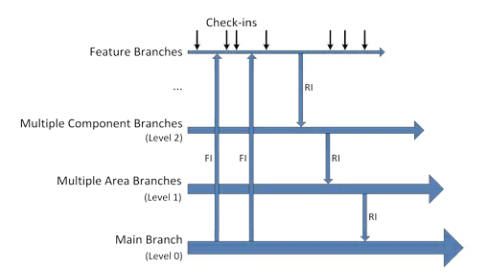
\includegraphics[scale=1]{microsoft-branching.png}
\end{center}
\caption[Voorbeeld flow]{Flow zoals vermeld in het artikel van  \textcite{Bird2012}}\label{fig_mic_flow}
\end{figure}

Elke ontwikkelaar schrijft zijn code op een feature branch. Het risico hiervan is dat men op den duur niet meer compatibel is met de hoofdboom. Er kunnen sinds de vertakking immers verschillende andere versies gepubliceerd zijn. Daarom wordt gewerkt met twee tussenbranches. Hier test men of de code compatibel is met de verschillende andere onderdelen van de software. Het proces waarbij men feature branches integreert in andere tussenbranches noemt men ook wel \textbf{Reverse integration} -aangeduid als RI op de figuur-. Een ander principe dat gebruikt wordt is dat van \textbf{Forward integration}. Hierbij worden de nieuwe versies van de hoofdbranch (ook wel master genoemd) geplaatst op de feature branch. Zo blijft de feature branch compatibel met alle veranderingen.

%toevoegen van GIT Flow
%toevoegen van Trunk based developmet
Buiten de methodiek voorgesteld door \textcite{Bird2012} bestaat er ook GIT Flow en Trunk based development. 


%\subsection{GIT}
%\label{sec:GIT}

\subsection{Conclusie}
\label{vb_conclusie}
De verschillende types van versiebeheersystemen -zoals besproken in \ref{sec:vb_inleiding}- hebben een gemeenschappelijke eigenschap. De bestanden en in veel gevallen het archief staan integraal opgeslagen op computers. Bij lokale versiebeheersystemen en CVCS staat het zelfs op één centrale computer. Dit introduceert het probleem van een SPOF (Single point of failure).DVCS vermijdt dit probleem door gebruikers kopieën te geven van het archief. Valt de centrale computer weg dan heeft elke gebruiker een back-up. Veranderingen tussen lokale versies en die op de centrale computer moet manueel gesynchroniseerd worden. Hierdoor heeft men in grote mate controle over wat er centraal wordt opgenomen. Het nadeel is dat er veel lokale kopieën zijn en veranderingen niet altijd worden gesynchroniseerd. Op deze manier heeft niet iedereen toegang tot de laatste veranderingen. Het zou dus een verbetering zijn mocht er een systeem bestaan dat één centraal archief ondersteunt zonder SPOF. Dit lijkt op eerste zicht niet mogelijk, aangezien er één centraal aanspreekpunt moet zijn. Toch is dit probleem al eerder opgelost onder de vorm van peer-to-peer (afgekort tot p2p) netwerken.\\

P2P is voornamelijk bekend onder de vorm van file-sharing netwerken zoals Napster. \textcite{Chawathe2003} stellen dat Napster één van de eerste systemen was die erin slaagde om een succesvol netwerk uit te bouwen. Bij dit netwerk worden files niet opgevraagd aan een centrale server. In plaats hiervan gebruikt men een netwerk van \textbf{peers}. Door de principes van dit type van netwerken toe te passen kan men een centraal archief op een gedistribueerde manier opslaan. Zo behoudt men het voordeel van CVCS zonder een SPOF. \\

De doelstelling van deze bachelorproef is om een werkend P2P versiebeheersysteem te gaan implementeren. Hiervoor moet men afbakenen welke functionaliteiten deze implementatie moet voorzien. In vorige paragrafen werden de verschillende concepten besproken. Hieronder volgt een oplijsting van deze verschillende concepten alsook een korte uitleg. Hierbij worden de terminologie en concepten van Git gebruikt. Deze worden vervolgens meegenomen naar volgende hoofdstukken, waar een implementatie wordt voorzien.

\begin{table}[h!]
	\centering
	\begin{tabular}{ |p{2cm}|p{12cm}|}
 		\hline
 		\multicolumn{2}{|c|}{\large \textbf{Concepten binnen versiebeheer}} \\
 		\hline
 		\textbf{Begrip}	& \textbf{Uitleg}\\
 		\hline
 		\textbf{Archief} & Een centrale plaats voor het bijhouden van bestanden. De wijzigingen van deze gearchiveerde bestanden worden bijgehouden. Men kan zowel historische als recente versies van het bestand opvragen alsook van het gehele archief.\\
 		\hline
 		\textbf{Versies} & Elke wijziging binnen het archief leidt tot een nieuwe versie. Men kan de verschillende versies ten alle tijden raadplegen. Men kan ook oudere versies gebruiken voor branching. In extreme gevallen kan een archief volledig worden teruggedraaid naar een eerdere versie.\\
 		\hline
		\textbf{Logboek} & Een bestand waarin alle wijzigingen worden bijgehouden. Het logboek is ook onderdeel van het archief. \\
		\hline
		Pushing	& Het principe waarbij wijzigingen die lokaal worden aangebracht, worden gesynchroniseerd met de centrale server.\\
		\hline
		Pulling & Het binnenhalen van veranderingen aangebracht op het centraal archief naar een lokale kopie.\\
		\hline
		Clonen & Het aanmaken van een lokale kopie van een centraal archief. \\
		Branching & Het voorzien van alternatieve vertakkingen van het archief. \\
		\hline
	\end{tabular}
	\label{tbl_concepts}
	\caption{Concepten binnen versiebeheersystemen.}
\end{table}
\newpage
\section{IPFS}
\label{IPFS}
\subsection{Het begrip decentralisatie}
\label{ipfs_decent}
De opzet van deze bachelorproef is om een volwaardig gedecentraliseerd versiebeheersysteem te bekomen door middel van P2P en blockchain technologie. Om de opzet volledig duidelijk te maken, moet het begrip \textit{"decentralisatie"} gekaderd worden. Stel onderstaand scenario:\\

Bob is een liefhebber van Capybaras en wil informatie krijgen over de dieren. Hij surft bijgevolg naar de Wikipedia pagina. Bob zal een verzoek moeten sturen naar de server van Wikipedia. Hiervoor moet hij het publieke IP-Adres kennen. Dit kan hij verkrijgen door het DNS protocol. Bob stuurt zijn verzoek naar deze server en krijgt de gezochte pagina terug. Dit is een voorbeeld van een gecentraliseerd systeem. Bob gaat immers op zoek naar één aanspreekpunt waar de informatie zich bevindt. Aangezien alle informatie zich bevindt op één plaats kan er worden gesproken van een gecentraliseerd systeem.\\

De manier van alle informatie op één punt te bewaren is effectief. Bob kan alle informatie snel en doeltreffend opvragen. Wat zijn echter de nadelen van deze manier van werken?

\begin{itemize}
	\item Een nadeel van dit centraal punt is het zogenaamde SPOF probleem -zie \ref{vb_conclusie}-. Doordat alle informatie zich op één server bevindt is er ook één kritieke plaats waar alles kan fout lopen. Is de server onbeschikbaar zijn alle diensten en informatie hierop dat ook.\\
	
	\item Doordat al het verkeer moet verwerkt worden door dezelfde hardware kan dit leiden tot een hoge serverbelasting. Hierdoor kan het verwerken van deze verzoeken traag verlopen.Om dit probleem op te lossen kan gebruik worden gemaakt van zogenaamde \textit{Mirror servers}. Dit is een kopie van de originele server. Deze kopie kan op momenten van hoge belasting een deel van het verkeer op zich nemen. Op die manier worden volgens \textcite{Webb2007} de beperkingen van bandbreedte die zich voordoen bij een klassiek server/client scenario geminimaliseerd. Toch is ook deze oplossing niet optimaal. Men heeft immers meerdere fysieke servers nodig en alle informatie is redundant. \\
	
	\item Het uitbreiden van bestaande infrastructuur is niet evident. Het verspreiden van een database over verschillende computers is een omslachtige onderneming.\\
		
	\item Een minder voor de hand liggend nadeel is dat van censuur. In sommige landen waaronder bijvoorbeeld China wordt bepaalde informatie gefilterd. Dit is mogelijk doordat deze landen het verkeer kunnen herleiden naar hun eigen servers.
\end{itemize}

De bovenstaande problemen worden aangepakt binnen het domein van \textbf{Distributed Computing}. Dit begrip wordt verder uitgelegd door \textcite{Attiya2004}: Distributed computing is een collectie van individuele computers die verbonden zitten in een netwerk en met elkaar kunnen communiceren. Deze computers zijn in staat om samen computermatige taken uit te voeren. \textbf{Peer-to-Peer}(afkort als P2P) is een principe dat kadert binnen dit begrip. Een gangbare definitie wordt gegeven door \textcite{Schollmeier2001}. Hij stelt dat Peer-to-peer een vorm is van distributed computing waarbinnen elke computer optreedt als een Servent. Dit is een combinatie van het woord \textbf{ser}ver en cli\textbf{ent}. Elke computer op dit netwerk is aldus in staat om verzoeken te behandelen en versturen. Dit staat haaks op de klassieke server-client benadering. \\

Peer-to-peer netwerken proberen om alle bovenstaande problemen met klassieke server-client netwerken systematisch op te lossen. Hoe doen ze dit exact?

\begin{itemize}
	\item Peer-to-peer netwerken zijn volstrekt gedecentraliseerd. Er is niet één computer die optreedt als server. Elke deelnemer van het netwerk (ook wel \textbf{Peer} genoemd) treedt op als server en client. Hierdoor is er geen SPOF.\\
	\item Hetzelfde principe geldt ook voor serverbelasting. Het gehele netwerk verwerkt immers verzoeken. Toch speelt data redundantie ook hier een rol. Een computer kan immers offline gaan en alle relevante informatie moet beschikbaar blijven.\\
	\item Een p2p netwerk is goed uitbreidbaar. Op elk moment kunnen computers toetreden tot het netwerk of uittreden.
\end{itemize}

Tot slot is het belangrijk om te vermelden dat er volgens \textcite{Schollmeier2001} twee verschillende categorieën zijn:

\begin{itemize}
\item De zogenaamde \textbf{pure netwerken} hierbij is elke computer gelijkwaardig. Met andere woorden men kan willekeurig welke deelnemer(Peer) uitschakelen en het netwerk zal nog op dezelfde manier functioneren.\\

\item Een netwerk waarbinnen er één centrale computer of een groep van computers zonder wie het netwerk niet functioneert wordt er gesproken van een \textbf{Hybride netwerk}
\end{itemize}


\subsection{De meerwaarde van decentralisatie binnen versiebeheer}
In \ref{ipfs_decent} worden decentralisatie en P2P kort toegelicht. In dit onderdeel ligt de focus op hoe deze principes kunnen worden toegepast binnen versiebeheersystemen.\\

In eerste instantie lijken sommige versiebeheersystemen gedecentraliseerd. \textbf{DVCS} is hier een goed voorbeeld van. Dit is een versiebeheersysteem waarbij elke computer een lokale kopie heeft van het centraal archief. Wijzigingen aan bestanden worden dan ook lokaal opgenomen. Elk lokaal archief is in staat om de functies als centraal archief op zich te nemen. Hierbij lijkt elke computer in staat om de functie van Servlet te vervullen en vertoont dit type van archief veel gelijkenissen met een P2P netwerk. Toch is er een eigenschap waaraan niet wordt voldaan; elk archief is immers niet gelijkwaardig. Er is altijd een centrale plaats waarvan de andere archieven worden gekopieerd.\\

DVCS heeft ook nog een aantal problemen die worden opgelost binnen een puur P2P netwerk. Er zijn verschillende lokale kopieën van een archief die niet noodzakelijk up-to-date zijn of waar de veranderingen niet zijn gesynchroniseerd. Als één van die computers wegvalt, zijn alle wijzigingen aangebracht in het lokaal archief ook verloren. 

Het begrip van een peer-to-peer netwerk is essentieel voor het maken van een gedecentraliseerd versiebeheersysteem. Binnen deze bachelorproef wordt er gebruik gemaakt van zo een netwerk voor twee verschillende doeleinden:

\begin{itemize}
\item Het opslaan van bestanden: de uiteindelijke doelstelling van een versiebeheersysteem is uiteraard om een archief te voorzien voor het behouden van wijzigingen aan bestanden. Deze bestanden moeten echter ergens worden bewaard. Mochten deze bestanden enkel lokaal worden opgeslagen dan is er het risico groot dat deze verloren gaan. Om dit tegen te gaan moet er een manier voorzien worden om bestanden op te slaan op een netwerk. Het meest bekende protocol voor gedecentraliseerde opslag is het torrenting protocol -voor meer informatie over een recente versie van dit protocol zie \autocite{Cohen2008}-. Torrenting maakt echter gebruik van een hybride netwerk. Er zijn verschillende protocollen die gebruik maken van compleet P2P. Een gekend voorbeeld hiervan is Gnutella -zie \autocite{Klingberg2002}-. Dit protocol is echter verouderd en wordt niet meer onderhouden. Een modern alternatief is \textbf{IPFS}.\\

\item Het opslaan van transacties: indien Alice een nieuwe versie van een bestand wilt publiceren moet Bob hiervan op de hoogte zijn. Er moet dus een manier zijn om informatie over te brengen naar elkaar. Hiervoor wordt er gebruik gemaakt van een blockchain. Een blockchain biedt een manier om informatieoverdracht mogelijk te maken op een P2P netwerk waarbij data integriteit wordt gewaarborgd. 
\end{itemize}

Het is ook belangrijk om kort te vermelden dat file-sharing controversieel is. Zo is de gekende Torrent indexering website \textit{"The Pirate Bay"} sinds 2011 verboden in België. Dit verbod is er gekomen aangezien file-sharing ook wordt gebruik voor het verspreiden van auteursrechtelijk beschermd materiaal. Niet alleen het Torrent protocol is hiervoor onder vuur komen te staan. Limewire een muziek deel platform gemaakt bovenop Gnutella werd in 2010 verplicht om te sluiten. Het probleem met deze maatregelen is dat ze niet kunnen worden doorgevoerd. Men kan individuele sites namelijk  blokkeren maar doordat de protocollen bovenop P2P netwerken zijn gebouwd is het niet mogelijk ze compleet onbeschikbaar te maken. Er zijn verschillende kopieën van de piratebay nog steeds toegankelijk in België en alternatieve versies van Limewire zijn eveneens beschikbaar. Het is hierbij belangrijk om te onthouden dat de principes en protocollen niet illegaal zijn maar het verspreiden van auteursrechtelijk beschermd materiaal is dat wel.\\

\subsection{bestandsopslag}
Voor de bestandsopslag zal gebruik worden gemaakt van IPFS. Dit deel wil een antwoord bieden op drie verschillende vragen:\\
Waarom wordt er gebruik gemaakt van een Protocol ten opzichte van een eigen implementatie?\\
Waarom worden BitTorrent en Gnutella besproken? 
\\Waarom de keuze voor IPFS ten opzichte van een ouder en meer getest protocol? Om de laatste vraag te beantwoorden worden de beperkingen en nadelen van de twee andere protocollen kort besproken.\\

Er wordt gebruik gemaakt van een reeds bestaand protocol aangezien P2P netwerken één grote beperking kennen: er is een groot aantal deelnemers nodig om het netwerk betrouwbaar te laten functioneren. Stel dat er slecht vijf computers in een netwerk zitten, dan is het niet onmogelijk dat al deze computers offline gaan. Hierdoor is het netwerk onbereikbaar. Een ander probleem binnen file-sharing netwerken is het principe van \textbf{ratio}. Binnen file-sharing Torrent protocollen kent men het onderscheid tussen een \textbf{Leecher} en een \textbf{Seeder}. Een peer die een bestand download wordt ook wel een Leecher genoemd en een node die een bestand beschikbaar stelt voor deze Leechers noemen we een Seeder. De ratio is bijgevolg het aantal seeders ten opzichte van het aantal leechers. Bij veel niet gesuperviseerde netwerken is dit ratio eerder laag -sommige netwerken legen namelijk verplichtingen op aan deelnemers zodat bestanden vlot toegankelijk blijven-. Veel leechers kiezen er namelijk voor om enkel bestanden te downloaden. Indien er geen Seeders meer zijn voor een bestand is dit in essentie ontoegankelijk geworden. Deze problemen kunnen worden vermeden door een voldoende groot netwerk te kiezen. Dit probleem doet zich echter ook voor bij protocollen zoals Gnutella en IPFS. Er is namelijk geen verplichting om bestanden beschikbaar te stellen. Eenmaal de peer de gewenste bestanden heeft binnen gehaald is er geen stimulans meer deze te delen. Het is dan ook aangewezen om een groot aantal deelnemers te hebben. Hoe meer Peers binnen een netwerk hoe meer toegankelijk het wordt en hoe meer kans dat deze peers ook effectief bestanden zullen beschikbaar stellen. Vandaar dat het aangewezen is om een reeds bestaand netwerk te gebruiken ten opzichte van een eigen implementatie.\\

Dit gedeelte biedt een korte inleiding over Gnutella en BitTorrent. Deze twee protocollen zijn interessant aangezien ze beide file-sharing binnen een P2P netwerk als einddoel, maar een volledig andere benadering hebben. Veel van de elementen en problemen die deze protocollen aanpakken,komen ook aan bod binnen IPFS. De vergelijking tussen BitTorrent en Gnutella biedt een meerwaarde aangezien het type netwerk dat elk gebruikt, verschilt. Zo kent men binnen BitTorrent het concept van Trackers. Dit is een centraal element waardoor men dus spreekt van een hybride netwerk. Gnutella heeft geen centraal element. Hier kan dus worden gesproken van een puur P2P netwerk.\\

Vóór de werking en nadelen van de verschillende protocollen kunnen worden uitgelegd is het belangrijk om even stil te staan bij het concept van een hash. Deze functie ligt aan de basis van het verifiëren van de dataintegriteit bij bestanden. Het concept speelt ook een grote rol binnen IPFS en Blockchain. Het is immers belangrijk om te kunnen nagaan of het bestand of data dat verkregen is hetzelfde is als wat verwacht wordt. Op deze manier kan er worden nagegaan of de data eventueel beschadigd zijn door de overdracht. Een ander probleem dat kan worden tegengegaan, is dat een peer probeert om kwadaardige bestanden te verspreiden waaronder malware. Een \textit{goede} hashfunctie zou moeten voldoen aan volgende eigenschappen (\autocite{Anderson93}):

\begin{itemize}
\item One-way functie: het is relatief eenvoudig om voor een gegeven dataset $x$ een resultaat te vinden $f(x)$. Het is echter onwaarschijnlijk om voor een gegeven resultaat $f(x)$ de originele dataset $x$ te vinden. Op deze manier is het makkelijk om een dataset te valideren indien de hashfunctie waarde gegeven.\\
\item Collision free: het moet niet mogelijk zijn dat twee verschillende datasets (bijvoorbeeld: $x$ en $y$) dezelfde hashfunctie waarde hebben. Wiskundig kan dit worden voorgesteld door volgende notatie:Stel een functie $f:A->B$. Deze functie is collision free indien $\forall \{x,y\}|\{x,y\} \subseteq A | f(x) \neq f(y)$\\
\item Gelijke verdeling: een kleine verandering aan de dataset leid tot een volledig verschillende hashwaarde. Zo is hashwaarde voor 123 en 124 sterk verschillend. Op deze manier kan er geen informatie worden afgeleid uit de hashwaarde zelf.\\
\item Vaste grootte: ongeacht de grootte van de ingegeven dataset, het resultaat van de lengte van de hash-functie is constant. Zo zal een MD5 Hash altijd 128 bit lang zijn ongeacht of de ingegeven data 1 bit of 10000 bits beslaat.
\end{itemize}
 
 \subsubsection{Torrenting}
Het BitTorrent protocol is wijd verspreid. Een studie door \textcite{Wang2013} stelt dat het dagelijks aantal van BitTorrent gebruikers tussen de 15-27 miljoen zit. Volgens de makers is de opzet ervan om een gangbaar alternatief te voorzien voor FTP. De uitleg van het protocol is gebaseerd op de tekst door \textcite{Fonseca2005}.\\ 

Het Torrent protocol bestaat uit drie delen. Het eerste deel is het verkrijgen van een \textbf{metainfo} bestand.\\

\begin{figure}[h!]
\centering
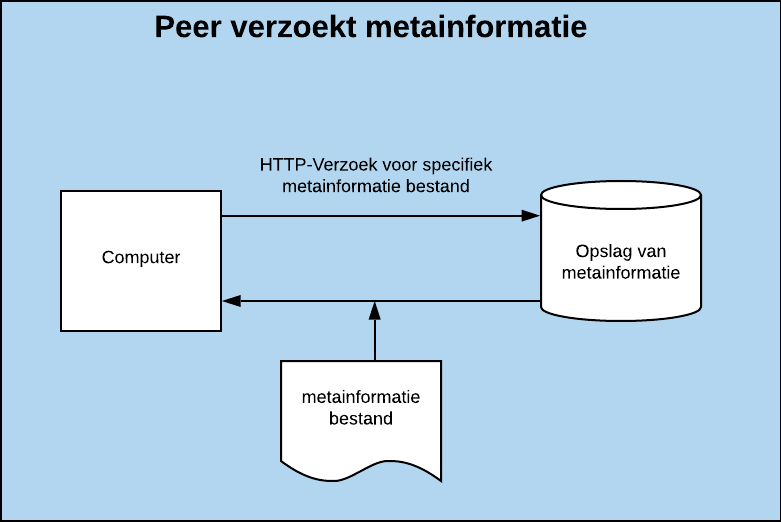
\includegraphics[scale=.4]{torrent-1.png}
\caption[Peer metainformatie stap  - Torrenting 1]{De peer maakt een verzoek aan een opslagplaats voor een metainformatie bestand.}
\end{figure}

Dit metainfo bestand wordt over het algemeen afgehaald van een website of een ftp server. Een gekend voorbeeld van een website die metainfo bestanden ter beschikking stelt is \textit{The pirate bay}. Dit bestand bevat essentiële informatie om de rest van het protocol te faciliteren. Het bevat de namen en bestandsstructuur van de verschillende bestanden binnen deze Torrent. Voor elk van deze bestanden is ook een MD5-Hashwaarde voorzien zodat eenmaal het bestand gedownload is de gebruiker kan controleren of het niet beschadigd is geraakt bij het download proces. Er wordt ook een zogenaamde infowaarde en stuklengte voorzien. Deze komen later aanbod. Het belangrijkste element in het metainfo bestand is echter het IP-adres van de \textbf{Tracker}. Deze Tracker is een computer die de andere delen van het protocol gaat overzien en aansturen. Aangezien er één centrale computer nodig is om dit protocol in goede banen te leiden is er dan ook sprake van een hybride netwerk.\\

\begin{figure}[h!]
	\centering
		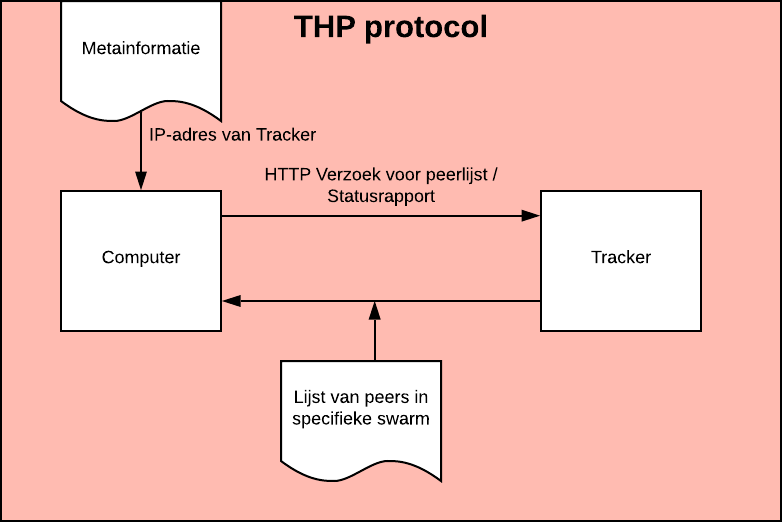
\includegraphics[scale=.4]{torrent-2.png}
			\caption[THP stap - Torrenting 2]{De peer doet een verzoek voor de peerlijst aan de tracker doormiddel van informatie uit het metainformatie bestand.}
\end{figure}
\newpage
Om deze stap te verduidelijken kan er gebruik worden gemaakt van volgend voorbeeld:\\

Bob en Alice maken een Torrent van hun website. Hun website bevat verschillende pagina's en afbeeldingen die zich in een media folder bevinden. Ze stellen een lijst op van deze verschillende bestanden en berekenen voor elk van deze bestanden een MD5-Hash waarde. Bobs computer zal de rest van het protocol coördineren en aldus functioneren als Tracker. Er wordt tot slot een unieke infosleutel voorzien en stuklengte (het is aangeraden deze stuklengte rond 70kb in te stellen). Op basis van deze informatie wordt een metainfo bestand aangemaakt dat wordt beschikbaar gesteld aan de buitenwereld.\\

In de volgende stap wilt men toegang verkrijgen tot andere peers die dit bestand bezitten. Men heeft immers andere computers nodig vanwaar men het bestand kan downloaden. De verzameling van computers die een torrent toegankelijk stellen voor het netwerk wordt ook wel een \textbf{swarm} genoemd. Men kan een swarm dan ook zien als een klein netwerk met als functie toegang te verlenen tot een specifieke collectie van bestanden. De functie van de Tracker is om toegang te verschaffen aan deze Swarm en ook informatie hierover bij te houden. Het principe van toegang verschaffen en informatie bijhouden wordt ook wel \textit{THP}(Tracker HTTP protocol) genoemd. De locatie van deze tracker staat vermeld in het metainfo bestand. Om een lijst van peers te krijgen die in een swarm zit, stuurt de computer een HTTP-GET verzoek naar de tracker. In dit verzoek moeten een aantal zaken worden meegestuurd waaronder het IP-adres van de computer, de infosleutel en de poort waarop de communicatie met andere peers kan gebeuren. De Tracker zal vervolgens aan de hand van de infosleutel een lijst van peers terugsturen die de gegeven bestanden ter beschikking stellen.\\

\begin{figure}[h!]
	\centering
		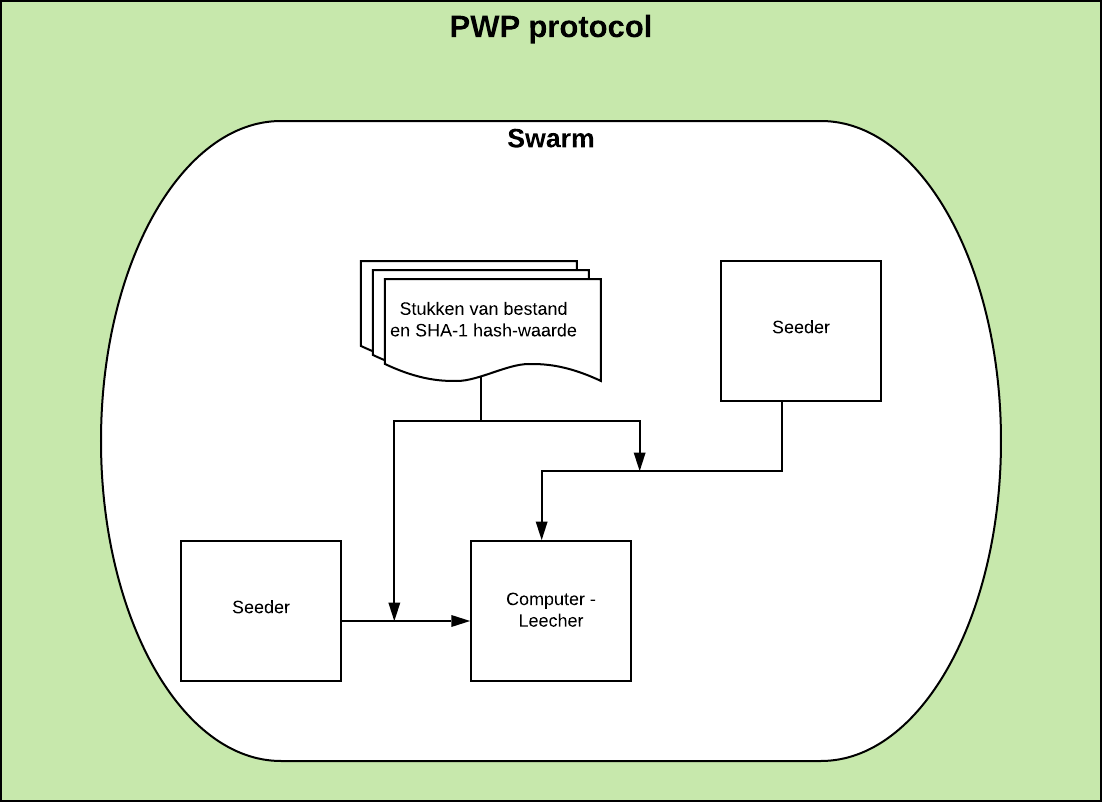
\includegraphics[scale=0.6]{torrent-3.png}
	\caption[PWP stap - Torrenting 3]{De peer verzoekt andere peers voor stukken data en downloadt op die manier de Torrent bestanden.}
\end{figure}
\newpage
Om dit principe te verduidelijken wordt verder gebouwd op bovenstaand voorbeeld:\\

Charlie wil de website van Bob en Alice. Hij heeft van Alice het metainfo bestand ontvangen. Aangezien dit bestand het IP-adres van Bobs computer als Tracker bestempelt wordt er naar deze computer een HTTP-GET verzoek verstuurd. Bob en Alice hebben beiden deze bestanden lokaal staan en vormen aldus samen een swarm. Charlie zal hun IP-adres en poort waarop het verkeer kan verlopen doorgestuurd krijgen en gaat rechtstreeks met beide computers communiceren om de bestanden te downloaden.\\

Opmerking: netwerken en bestanden zijn erg veranderlijk, een computer kan elk moment uitgaan of van het netwerk treden. Het is dus noodzakelijk dat de Tracker een accurate lijst van peers gaat bijhouden in de Swarm. Om dit te bereiken zal een Tracker vragen dat elke peer op een vast tijdsinterval zijn status gaat rapporteren. Zo kan de Tracker accurate informatie voorzien.\\

De computer heeft nu een lijst van verschillende Peers binnen een specifieke swarm. De laatste stap van het protocol is het effectief verkrijgen van de bestanden. De communicatie loopt uitsluitend tussen de verschillende peers zelf. Deze stap wordt ook wel aangeduid als het \textit{PWP} protocol (Peer Wire Message). Bandbreedte en andere beperkingen spelen een grote rol binnen netwerkverkeer. Men wil een peer zo weinig mogelijk belasten. Op die manier stimuleert men de peer om zolang mogelijk op het netwerk te blijven. Het is aldus niet praktisch om volledige bestanden op te vragen van één peer. Stel dat het bestand bijvoorbeeld verschillende gigabytes groot is. Hierdoor zal men het bestand opdelen in verschillende kleine stukken. Deze stukken kunnen individueel worden opgevraagd aan verschillende computers. Op deze manier kan men een bestand van verschillende gigabytes in duizend keer opvragen bij verschillende peers die elk enkele mb doorsturen. De grootte van elk stuk wordt bepaald in het metainfo bestand en staat vastgelegd in de zogenaamde stuklengte. Een ander voordeel van deze fragmentering is dat men individuele stukken kan verifiëren. Elk van deze stukken heeft namelijk zijn eigen SHA-1 hashwaarde. Op die manier kan men gedurende de overdracht van een stuk onmiddellijk nagaan of dit goed is toegekomen en indien er fouten zijn dit klein stuk opnieuw opvragen. Het PWP protocol komt neer op het opvragen en valideren van individuele stukken aan verschillende peers.\footnote{De manier waarop deze stukken worden opgevraagd, ligt buiten de scope van deze bachelorproef. Een goed overzicht wordt gegeven in de tekst van \textcite{Fonseca2005}.} Eenmaal alle stukken zijn gedownload, worden deze samengenomen tot het origineel bestand dat opzijn beurt kan worden gevalideerd aan de hand van MD5.

%vermeld dat bittorrent seed terwijl de download bezig is

\subsection{Hoe worden bestanden geïdentificeerd op het netwerk}
Een probleem binnen file sharing is de wijze waarop men bestanden opvraagt. Dit kan het best worden geïllustreerd aan de hand van een voorbeeld.\\

Alice wilt graag een afbeelding van de paashaas. Na het opzoek door middel van een zoek machine vind ze deze afbeeldingen op een gegeven URL. Deze URL is verbonden aan een server die op zijn beurt de afbeelding bevat. Alice kan dus eenvoudigweg de afbeelding daar opvragen. Op een gedecentraliseerd systeem is dit niet evident er is immers geen server waar bestanden ter beschikking staan. De bestanden zitten namelijk verspreid over verschillende computers. Toch moet het systeem instaat zijn om bestanden terug te vinden.\\

Om dit probleem op te lossen wordt er niet naar een specifieke plaats genavigeerd zoals met een URL. Het netwerk wordt rechtstreeks bevraagd voor een bestand. De peers die dit bestand ter beschikking hebben zullen dit bestand doorsturen naar de peer die het heeft opgevraagd. Voor dit principe heeft elk bestand een uniek identificatie nummer nodig. Een bestandsnaam is immers niet uniek.\\

Hiervoor kan men gebruik maken van \textbf{Hashfuncties}. Een hashfunctie is een wiskundige functie die aan een
